\subsection{Starting Fresh}
\label{sec:loadSourceMeta}
\begin{itemize}

\item[$\blacktriangleright$] Press the \texttt{new} button on the Eclipse toolbar and navigate to ``Examples/eMoflon Handbook Examples/''
(Fig.~\ref{eclipse:downPartIV}). There are two \texttt{Part IVFresh Start} cheat packages: one for our visual syntax, the other for our textual
syntax. They each contain the full \texttt{LeitnersLearningBox} metamodel, as well as each method implemented as an SDM and an exemplary instance of the
metamodel. If you need help deciding which syntax to use, refer to Part I, Section 1.

\begin{figure}[htbp]
\begin{center}
  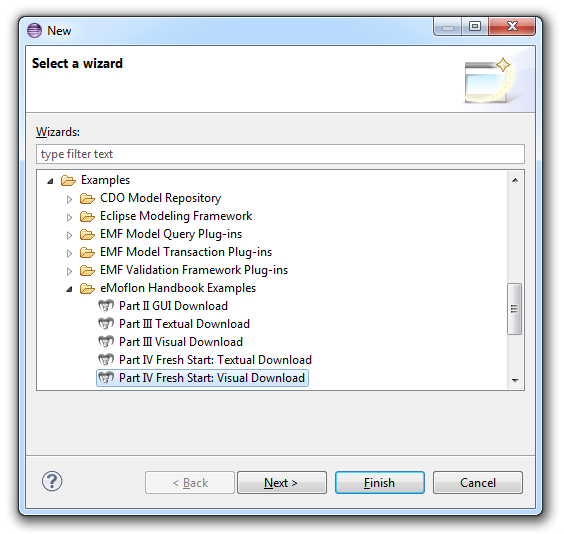
\includegraphics[width=0.65\textwidth]{eclipse_part4FreshWizardDownload}
  \caption{Initialize your workspace with your preferred syntax}
  \label{eclipse:downPartIV}
\end{center}
\end{figure}

\vspace{0.5cm}

\item[$\blacktriangleright$] After loading, if your package explorer does not resemble ours in Fig.~\ref{eclipse:workingSets} with at least two distinct nodes,
select the small, downward facing arrow in the corner of the package explorer. Choose ``Top Level Elements/Working Sets.'' To review how these nodes are used
to structure our workspace in Eclipse, check out Part I, Section 4.

\vspace{0.5cm}

\begin{figure}[htbp]
	\centering
  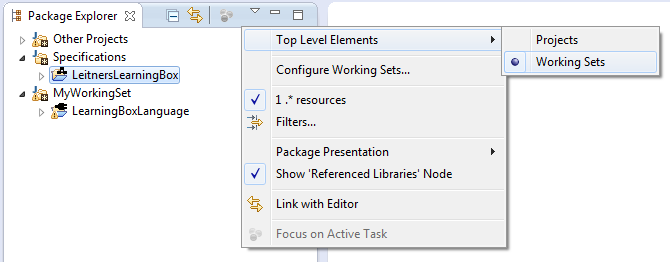
\includegraphics[width=0.9\textwidth]{eclipse_workingSets}
	\caption{Setting your Package Explorer}
	\label{eclipse:workingSets}
\end{figure}

\vspace{0.5cm}

\item[$\blacktriangleright$] Fantastic -- you now have the source metamodel for your transformation ready to go!

\end{itemize}